\chapter{Bomba de infusão de insulina}
\section{Contextualização}
Glicose, a principal fonte de energia do corpo humano, é absorvida a partir dos alimentos e distribuída ao corpo através da corrente sanguínea. Uma vez que está no sangue ela pode ser absorvida pelo fígado, temporariamente, utilizada pela células ou, em último caso, ser eliminada através da urina. Processos do corpo regulados pelos hormônios, que mantém a quantidade de glicose estável na corrente sanguínea. Dos hormônios existentes os mais importante é a insulina. Sua produção é feita pelo pâncres e sua função é controlar absorção de glicose pelas células \cite{sbc2014}

Segundo \cite{sbc2014} existem conjunto de doenças crônicas, chamadas diabetes, que dificultam o metabolismo da glicose e da insulina. A diagnósticação dessa doença geralmente pode ser feita através da aferição da concentração de glicose na corrente sanguínea. O resultado positivo se dá em caso de ser constatado hiperglicemia, ou seja, elevada concentração de glicose.

Dentre os tipos de diabetes o mais raro é o tipo 1. O paciente com esse tipo de doença faz com que seja necessário a aplicações diárias de insulina, consequência da secreção desse hormônio. Esse tipo da doença ocorre por causa desconhecida ou, ainda sim, pela destruição das células betas pelo pâncres, ocasionada por um processo auto-imune \cite{galvao2013requirements}. Os principais tipos tratamentos para o quadro citado são:
\begin{itemize}
\item Infusão Contínua Subcutânea de Insulina através de uma bomba de infusão, situação abordada neste trabalho;
\item Múltiplas Doses de Insulina (MDI).
\end{itemize}

\section{Características gerais da bomba de infusão}
Segundo \cite{minicucci2008uso}, para gerenciar o processo de infusão de insulina no paciente é utilizado um dispositivo eletrômecanico portátil conhecido como: bomba de insusão de insulina. A idéia desse aparelho é atuar como um pâncres artificial, ou seja, atuar de forma similar ao organismo de uma pessoa que não possui diabetes, liberando insulina durante o dia todo e no horário das refeições. A primeira forma de funcionamento, liberação de insulina entre as refeições, é chamada de basal e a segunda bolus.

A bomba geralmente é ligada a um tubo de plástico fino, cateter, que uma cânula flexível de teflon, colocada sob a pele do obdômen ou coxa. É posicionada externamente ao corpo e possui um peso entre 80 e 100 gramas. Além das posições citadas a bomba pode ser posicionada na região lombar ou até mesmo nos membros superiores \cite{minicucci2008uso}.

Segundo \cite{amorim2008novas}, o software embarcado, responsável pelo controle da bomba possui algumas funcionalidades como:

\begin{itemize}
\item avisos para monitoração da glicose;
\item programação de doses de taxas basais para cada hora do dia;
\item programação de doses de taxas bolus para certa quantidade de refeições;
\item possibilidade de bloqueio do sistema voltados principalmente para utilização em crianças;
\item possibilidade de escolha de menus operacionais;
\item programação de quantidade de insulina a ser injetada;
\item alarmes vibratórios e/ou sonoros para quantidade de insulina no reservatório;
\item avisos para monitoração da glicose;
\item ajuda de Bolus que auxilia no cálculo da dose bolus necessária para correção de hiperglicemia e/ou alimentação (essa funcionalidade mais difícil de ser encontrada);
\item dentre outras verificações de segurança.
\end{itemize}

Hoje em dia, a configurabilidade das funcionalidades da bomba de infusão é muito mais do que as funcionalidades básicas, o que aumentam seu custo e podem não agregar muito valor ao consumidor final. Funcionalidade essas como:

\begin{itemize}
\item integração com algum sistema de monitoração contínuo de glicose;
\item sistema bluetooth onde o paciente utiliza um dispositivo externo para o controle da bomba;
\item sistema de transferência de dados para um computador;
\item lembretes;
\item personalizações de menu;
\item gráficos;
\item visores coloridos;
\item entre outros.
\end{itemize}

\section{Aspectos de segurança da bomba de infusão}
A bomba de infusão é considerado um sistema embarcado de tempo real crítico uma vez que dever ser extremamente seguro e fornecer respostas em prazos precisos e determinados. Considerações essas que implicam em diferenças importantes de projeto em relação a sistemas mais simples, pois complicações em sistemas desse tipo podem causar até mesmo a morte. Logo, esses dispositivos devem ser desenvolvidos com critérios de segurança robustos e requisitos funcionais e não-funcionais bem definidos \cite{sommerville2004software}.

É importante que o sistema seja confiável ao fornecer a quantidade correta de insulina requisitada, ou seja, ter disponibilidade sempre que for requisitada e, não menos importante, a bomba deve ser segura tratando falhas que possam suspender o fornecimento de insulina ou a infusão demasiada da mesma. Segundo \cite{sommerville2004software}, todas as condições anteriores retratam alguns requisitos de sistemas críticos, que no contexto deste trabalho podem ser representados por algumas funcionalidades essenciais, tais como:

\begin{itemize}
\item Alarmes para o nível da bateria;
\item Sensor de pressão;
\item Redundância de partes do hardware essenciais;
\item Rotinas de verificação do funcionamento interno em geral (hardware e software);
\item Implementação de rotinas que prevêem iterações de forma errada por parte do paciente;
\item Inacessibilidade de algumas configurações avançadas por meio do paciente;
\item Alarmes para o nível de reservatório;
\item Hardware de boa qualidade com as devidas certificações.
\end{itemize}

Segundo \cite{zhang2010hazard} pode-se listar situações referentes ao uso da bomba que podem causar alguma falha, podendo levar o paciente a perder a consciência no caso de uma hipoglicemia e cetoacidose para uma considerável hiperglicemia. A divisão é feita em seis grupos principais: causas operacionais, falhas de software, falhas de hardware, causas ambientais, elétricas e químicas.

Levantamento este importantíssimo para servir como gui do projeto, de forma que se possa medir e garantir os mais altos níveis de segurança tanto no \emph{software} quanto no \emph{hardware}. Ainda existe classificações de riscos que podem ser energéticas, mecânicas, biológicas, químicas, ambiental e terapêutica \cite{zhang2010hazard}. 

Exemplos de causas operacionais que levam a situação de riscos:
\begin{itemize}
\item Bomba está desconectada do conjunto de infusão sem o conhecimento do paciente;
\item Excessiva administração da taxa de bolus devido a várias requisições do paciente;
\item Vazamento da bomba;
\item Taxa atual de infusão não está de acordo com o programado;
\end{itemize}

Exemplos de falhas de \emph{software} que levam a situação de riscos:
\begin{itemize}
\item \emph{Looping} infinito;
\item Acesso indevido da memória;
\item Taxa incorreta de bolus recomendada pelo cálculo do sistema;	
\item Estouro de pilha.
\end{itemize}

Exemplos de falhas de \emph{hardware} que levam a situação de riscos:
\begin{itemize}
\item Falha na memória ROM ou flash;
\item Falhas do motor;
\item Falha no sensor de reservatório de insulina;	
\item Falha no sensor de bateria;
\item Falha no microcontrolador.
\end{itemize}

Exemplos de causas ambientais que levam a situação de riscos:
\begin{itemize}
\item Aquecimento da bomba durante o funcionamento;
\item Alta diferença de pressão entre o interior da bomba e o ambiente externo;
\item Uso da bomba em temperaturas fora do especificado;
\item Uso da bomba em ambientes com alta umidade.
\end{itemize}

Exemplos de causas elétricas que levam a situação de riscos:
\begin{itemize}
\item Interferência eletromagnética vinda de outros aparelhos eletrônicos;
\item Bateria desconectada;
\item Vazamento de corrente pela superfície da bomba;
\item Nível de bateria baixo;
\item Descarga eletrostática.
\end{itemize}

Exemplos de causas químicas e/ou biológicas que levam a situação de riscos:
\begin{itemize}
\item Material do equipamento de baixa qualidade, problemas alérgicos;
\item Infecção na região (pele) da infusão;
\item Perda das propriedades bioquímicas da insulina durante a infusão, hiperglicemia;
\item Precipitação química dentro do cateter, problemas alérgicos, infecções;
\item Equipamento não higienizado, problemas alérgicos, infecções.
\end{itemize}

\section{Requisitos da bomba de infusão}

A bomba será implementada utilizando um microcontrolador de baixo custo da família PIC, de forma a manter as características mais importante, qualidade e segurança do dispositivo. A Figura \ref{fig:contextobomba} representa o modelo do contexto da bomba de infusão de insulidade, com todas as entidadesque deverão ser monitoradas e/ou controladas pelo software.

\begin{figure}[htp]
	\centering
	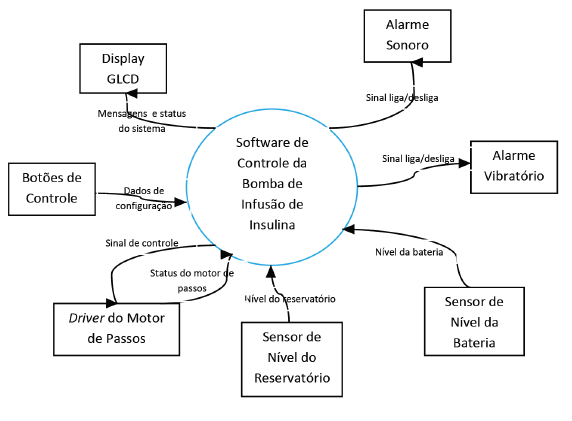
\includegraphics[scale=1]{images/contexto_bomba.png}
	\caption{Modelo de contexto da bomba de infusão de insulina}	
	\label{fig:contextobomba}
	\cite{galvao2013requirements}
\end{figure}

A divisão dos requisitos funcionas da bomba foi feita da seguinte forma:
\begin{itemize}
\item Módulo de interface com o usuário;
\item Módulo de controle de infusão;
\item Módulo de monitoramento de sensores.
\end{itemize}

Abaixo segue figuras para representar os módulos do sistema citados anteriormente. A Figura \ref{fig:usecaseinterfaceusuario} representa o móddulo de interface com o usuário, pode-se observar as possíveis ações que o usuário pode realizar de forma a interagir com o sistema. A Figura \ref{fig:usecasemoduloinfusao} representa o segundo módulo, controle de infusão, que tem a responsabilidade de administrar as duas formas de infusão: basal e bolus. O último, módulo de monitoramento dos sensores, está representado na Figuza \ref{fig:usecasemodulosensores} e é responsávels pela verificação do sistema como um todo.

\begin{figure}[htp]
	\centering
	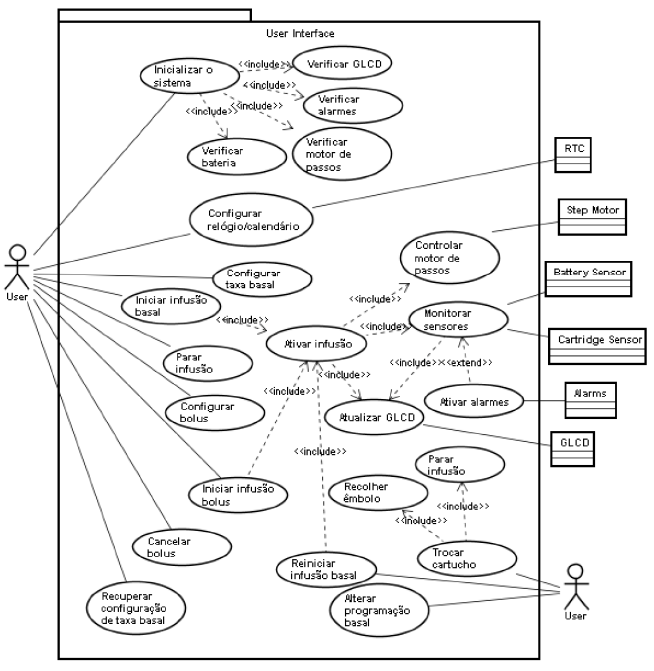
\includegraphics[scale=0.8]{images/caso_uso_interface_usuario.png}
	\caption{Caso de uso do módulo de interface com o usuário}	
	\label{fig:usecaseinterfaceusuario}
	\cite{galvao2013requirements}
\end{figure}

\begin{figure}[htp]
	\centering
	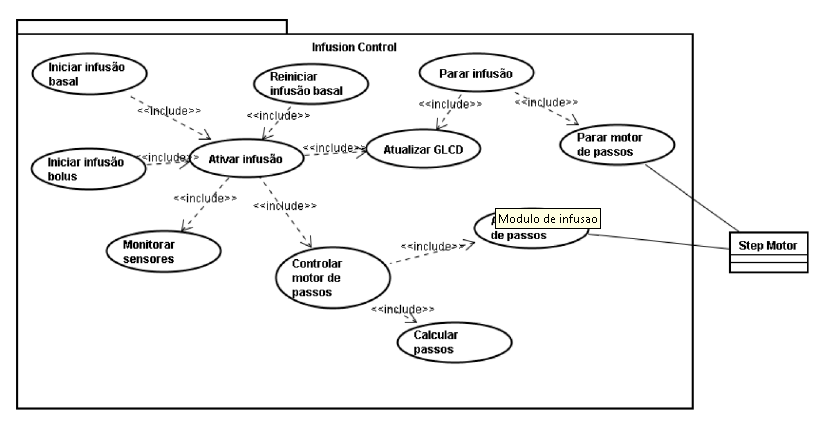
\includegraphics[scale=0.7]{images/modulo_infusao.png}
	\caption{Caso de uso do módulo de controle de infusão}	
	\label{fig:usecasemoduloinfusao}
	\cite{galvao2013requirements}
\end{figure}

\begin{figure}[htp]
	\centering
	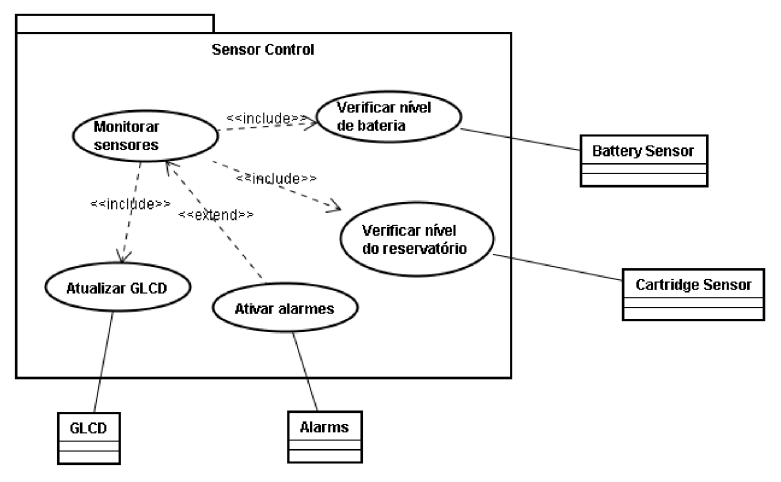
\includegraphics[scale=0.7]{images/modulo_sensores.png}
	\caption{Caso de uso do módulo de monitoramento dos sensores}	
	\label{fig:usecasemodulosensores}
	\cite{galvao2013requirements}
\end{figure}

